\documentclass[11pt,letterpaper]{article}

\usepackage[margin=1in]{geometry}
\usepackage{graphicx}
\usepackage{booktabs}
\usepackage{amsmath,amssymb}
\usepackage{hyperref}
\usepackage{xcolor}
\usepackage{microtype}
\usepackage{url}
\usepackage{enumitem}

\hypersetup{colorlinks=true,linkcolor=blue,citecolor=blue,urlcolor=blue}

\title{FabricCrypt: Software-Discoverable, Vendor-Key-Free Per-Die
       Attestation \emph{Primitive} for AI Inference on Commodity GPUs
       (at $n=2$ chassi)}
\author{E.\ Bergvall \\ \texttt{bergvall.eric@gmail.com}}
\date{Draft v3.1 --- \today}

\begin{document}
\maketitle

\begin{abstract}
We present \textbf{FabricCrypt}, a software-discoverable, vendor-key-free
per-die attestation \emph{primitive} (at $n=2$ chassi) demonstrated
end-to-end on commodity AMD hardware. FabricCrypt couples (i) a
466-dimensional live device signature assembled from \textbf{15 signals
total}---5 baseline HAL-bypass micro-architectural signals (TSC offsets,
cacheline ping-pong, DRAM-refresh jitter, syscall $p_{99.9}$ tails, NVMe
queue tails), 3 cross-host KS-verified micro-architectural signals from
Phase~19 (GPU clock jitter, multi-zone thermal spread, temporal-Jacobian
dynamics), and 7 board-level deterministic fingerprint signals from
Phase~22 (PCI/PCIe/USB/DMI/UCSI/amdgpu/kernel-boot)---with (ii) an
audience-supplied 64-bit nonce that drives the \emph{sampling plan
itself} (which CPUs, which thermal zones, which core pairs, which sleep
durations). On two AMD Ryzen AI Max+ 395 ``Strix Halo'' laptops we obtain
100\% leave-one-out per-die classification on the 466-dim extended
signature (gate $>0.95$) and pass all 10 protocol attack gates from the
v2.1 extended battery including the O115 custom forgery. End-to-end
sign-and-verify latency is sub-millisecond (median 1.12\,ms,
$p_{99}$ 2.79\,ms). Capability gains on two downstream tasks are large
and reproducible: anomaly-detection AUROC $0.500 \to 0.994$ and
host-attribution accuracy $0.501 \to 1.000$. Tier-2 cryptographic
hardening (Reverse Fuzzy Extractor~\cite{VanHerrewege2012},
Controlled-PUF wrap~\cite{Suh2007}, multi-round response protocol, ZK
inference-binding scaffold) provides \emph{empirical} operating points
(no formal cryptographic reduction): the Controlled-PUF wrap returns
Hamming $\mu = 128/256$ (random floor) against ML-modeling attackers
across $N_{\text{train}} \in \{50, 100, 150, 160\}$, i.e.\ $\geq 10^4$
modeling samples without measurable progress; Reverse-FE yields 0/100
imposter acceptance. \textbf{All bit-security figures in this paper are
empirical operating points, not formal proofs.} We have not shown:
(a) static-benchmark inference-accuracy gain (null); (b) chassis count
$n=2$; (c) the LAN-relay attacker (V6) defeats every Tier-2 mitigation
---distance bounding~\cite{Brands1993} is explicitly out of scope;
(d) the ZK inference-binding circuit is specified but not compiled.
FabricCrypt offers per-die attribution that the vendor-PKI-rooted
designs (Apple PCC, NVIDIA CC, Intel TDX, AMD SEV-SNP) do not, without a
Secure Enclave, TPM EK certificate, or any vendor key material---but the
demonstration is at $n=2$ chassi and the cryptographic ceilings are
empirical, not proven.
\end{abstract}

\section{Introduction}

Trustworthy AI inference is in the middle of a quiet PKI war.
Apple's Private Cloud Compute (PCC)~\cite{PCC2024} binds inference
attestation to a \emph{vendor} signing key rooted in a Secure Enclave.
NVIDIA Confidential Compute~\cite{NVIDIACC} binds H100/Blackwell
attestation to a DICE-rooted certificate signed by NVIDIA. Intel
TDX~\cite{TDX2024} and AMD SEV-SNP~\cite{SEVSNP} root attestation in
the silicon vendor's CA. All four share a property: \emph{if you do not
trust the vendor's PKI, you do not have attestation}. Worse, all four
authenticate the SKU class---``an H100 in confidential mode''---not the
individual die.

We ask: \emph{can commodity AMD hardware provide a per-die attestation
primitive (at $n=2$ chassi) without depending on the vendor's PKI?}\ Our
answer is yes, provided we bypass the HAL and read low-level
micro-architectural signals that PSP firmware does not (and cannot
cheaply) sanitize, \emph{and} combine them with board-level
deterministic fingerprints for zero-FP short-circuit identification.

\paragraph{Contributions.}
\begin{enumerate}[noitemsep,topsep=2pt]
\item \textbf{15 signals total} that together yield a 466-dimensional
      per-die fingerprint with 100\% LOO classification \emph{at $n=2$
      chassi}: 5 baseline HAL-bypass micro-architectural + 3 cross-host
      KS-verified micro-architectural (Phase~19,
      Bonferroni $p < 3{\times}10^{-3}$) + 7 board-level deterministic
      fingerprint signals (Phase~22, \emph{not} HAL-bypass).
\item A nonce-driven sampling plan that controls \emph{what gets
      measured}---defeating static and dynamic-library replay.
\item An all-ten-gate protocol battery including the post-disclosure
      O115 forgery; latency $<3$\,ms at $p_{99}$.
\item Tier-2 cryptographic hardening: Reverse Fuzzy
      Extractor~\cite{VanHerrewege2012} defeats helper-data leakage;
      Controlled-PUF wrap~\cite{Suh2007} defeats ML modeling attacks
      empirically (Hamming $\mu = 128$ at $\geq 10^4$ modeling samples,
      reproducing the~\cite{Ruhrmair2010} baseline); multi-round
      protocol forces full response-surface emulation; ZK
      inference-binding scaffold (Pedersen + HMAC) interface-ready for
      ezkl. \textbf{Operating points are reported as empirical
      attack-cost, not formal cryptographic reductions.}
\item Three new capabilities the vendor-PKI designs cannot provide:
      per-die output attribution, stateless PCC-equivalent guarantees
      on commodity AMD, and TEE-free sybil-resistant federated learning.
\item Honest residual-risk accounting at three adversary tiers, with
      Tier 2 (calibration-file capture) bounded by an empirical 3-round
      Mahalanobis emulator-accept of 0/100, \emph{not} by a formal
      reduction.
\end{enumerate}

We deliberately do \emph{not} claim a static-benchmark accuracy gain
from embodiment: it was pre-registered and came back null. We discuss
this honestly in Section~\ref{sec:limits}.

\section{Background and Related Work}

\paragraph{Hardware-rooted attestation.} PCC~\cite{PCC2024}, NVIDIA
CC~\cite{NVIDIACC}, TDX~\cite{TDX2024}, and SEV-SNP~\cite{SEVSNP} all
root attestation in the silicon vendor's CA and authenticate SKU class,
not individual die. TPM~2.0~\cite{TPM2} is per-platform but vendor-CA
rooted. LAMINATOR~\cite{LAMINATOR2025} provides certifiable ML
ownership but requires a TEE root; FabricCrypt is the
commodity-AMD, no-TEE analogue.
Eckel, Fenzl, J\"ager~\cite{EckelFenzlJaeger2024} demonstrated
embedded-ADC fingerprinting for remote attestation; FabricCrypt
generalises to a 15-signal bundle on commodity APUs without dedicated
ADC peripherals.

\paragraph{Substrate-as-identity.} DRAM Latency PUF~\cite{Kim2018},
DRAWNAPART~\cite{DRAWNAPART}, and FP-Rowhammer~\cite{Venugopalan2023}
treat micro-architectural noise as identity-bearing physical state.
FabricCrypt is challenge-bound and live where these are static.

\paragraph{Controlled PUFs and modeling attacks.}
Suh-Devadas~\cite{Suh2007} introduced the Controlled-PUF construction
in which a hash-based wrapper on the PUF response prevents a
model-building adversary from observing clean challenge-response pairs.
R\"uhrmair et al.~\cite{Ruhrmair2010} showed that arbiter and
ring-oscillator PUFs are uniformly vulnerable to ML modeling; this
motivates a hash-wrapped construction over any analog substrate.
Van Herrewege et al.~\cite{VanHerrewege2012} introduced the
\emph{Reverse} Fuzzy Extractor at FC'12, moving helper-data computation
server-side. FabricCrypt's Tier-2 hardening (Sec.~\ref{sec:tier2})
adopts both constructions directly.

\paragraph{Clock-skew identification.} Kohno et al.~\cite{Kohno2005}
showed TCP timestamp drift identifies devices across networks.
Sanchez-Rola et al.~\cite{SanchezRola2018} extended this to browser
timers. FabricCrypt generalises to 15 signals with a nonce-driven plan.

\paragraph{Frequency / power side channels.}
Hertzbleed~\cite{Hertzbleed2022} and Energon~\cite{Energon2025} treat
DVFS / power coupling as a leak. FabricCrypt inverts the polarity and
treats the same coupling as identity.

\section{Threat Model}

We consider three adversary classes:
(A) replay attackers with up to $10^5$ honest (nonce, signature) pairs;
(B) chip-cloning attackers at manufacturer scale;
(C) side-channel attackers reconstructing the fingerprint remotely.
The verifier is honest. The fingerprint is intentionally observable.
The protocol defends \emph{re-use} of an observed fingerprint, not
its observation. LAN-relay distance attacks (V6) are out of scope:
they require hardware distance bounding~\cite{Brands1993}.

\section{Identity Mechanism}

\subsection{Five HAL-bypass baseline signals}
\begin{itemize}[noitemsep,topsep=2pt]
\item \textbf{Task B}: inter-core TSC offset matrix (16 cores $\times$ 16).
\item \textbf{Task E}: MOESI cacheline ping-pong latency.
\item \textbf{DRAM-aligned jitter}: phase-locked latency under refresh.
\item \textbf{Syscall $p_{99.9}$ tails}: per-core scheduler tail
      under \texttt{SCHED\_FIFO}.
\item \textbf{NVMe queue-tail latency}: per-namespace submission jitter.
\end{itemize}
Concatenated and z-scored, these yield 290 dimensions.

\subsection{Three cross-host KS-verified micro-architectural signals (Phase 19)}
\begin{itemize}[noitemsep,topsep=2pt]
\item \textbf{S4 GPU clock jitter}: GPU PLL phase noise across 20 short
      kernel launches; Bonferroni-corrected $p < 3{\times}10^{-3}$.
\item \textbf{S6 Multi-zone thermal spread}: per-zone temperature
      delta under synchronized load; reflects board thermal geometry.
\item \textbf{S9 Temporal-Jacobian dynamics}: top-eigenvalue spectrum
      of a per-die input-output Jacobian on a short benchmark stream;
      defeats static-only adversaries.
\end{itemize}

\subsection{Seven board-level deterministic fingerprint signals (Phase 22)}
\label{sec:phase22}
These are \textbf{not HAL-bypass micro-architectural signals}; they are
\textbf{board-level deterministic fingerprints} of the printed-circuit
assembly around the APU. Within-host KS-D is exactly zero
(bit-identical across reps); cross-host accept is exactly zero false
positives unless the board layout is modified.

\begin{table}[h]
\centering\small
\begin{tabular}{lll}
\toprule
Signal & Source & Mechanism \\
\midrule
S20 PCI topology hash & \texttt{/sys/bus/pci/...} & per-board bus/dev/fn tree \\
S21 PCIe link state   & \texttt{lspci -vv}        & per-board PCIe negotiation \\
S22 USB descriptor    & \texttt{lsusb -v}         & per-board USB HID tree \\
S23 DMI/SMBIOS hash   & \texttt{/sys/class/dmi/} & UEFI store SHA-256 \\
S24 Kernel boot timing& \texttt{dmesg -T}         & firmware-to-kernel schedule \\
S25 UCSI PD VDM       & \texttt{/sys/class/typec/}& Type-C controller firmware \\
S26 amdgpu safe reads & non-mailbox regs          & per-die fuse-derived statics \\
\bottomrule
\end{tabular}
\caption{Phase 22 board-level deterministic fingerprints (S20--S26).
NOT HAL-bypass micro-architectural; bit-identical within host.}
\end{table}

\paragraph{Headline count: 5 HAL-bypass + 3 cross-host KS-verified $\mu$-arch + 7 board-level deterministic = 15 signals.}

\subsection{Signature\_v3: 466-dimensional extended signature}
The full v3 signature concatenates 15 signal families across three
classes: baseline (290), Phase 19 $\mu$-arch (72), Phase 22 board-level
(96), plus the stochastic S27 HPET/RTC drift (8) outside both headline
subgroups, for 466 dimensions total. Leave-one-out 1-NN cosine
classification at $n = 2$ hosts, 10 reps each, gives \textbf{LOO
accuracy $= 1.000$}. Figure~\ref{fig:sep} shows the separation.

\begin{figure}[t]
  \centering
  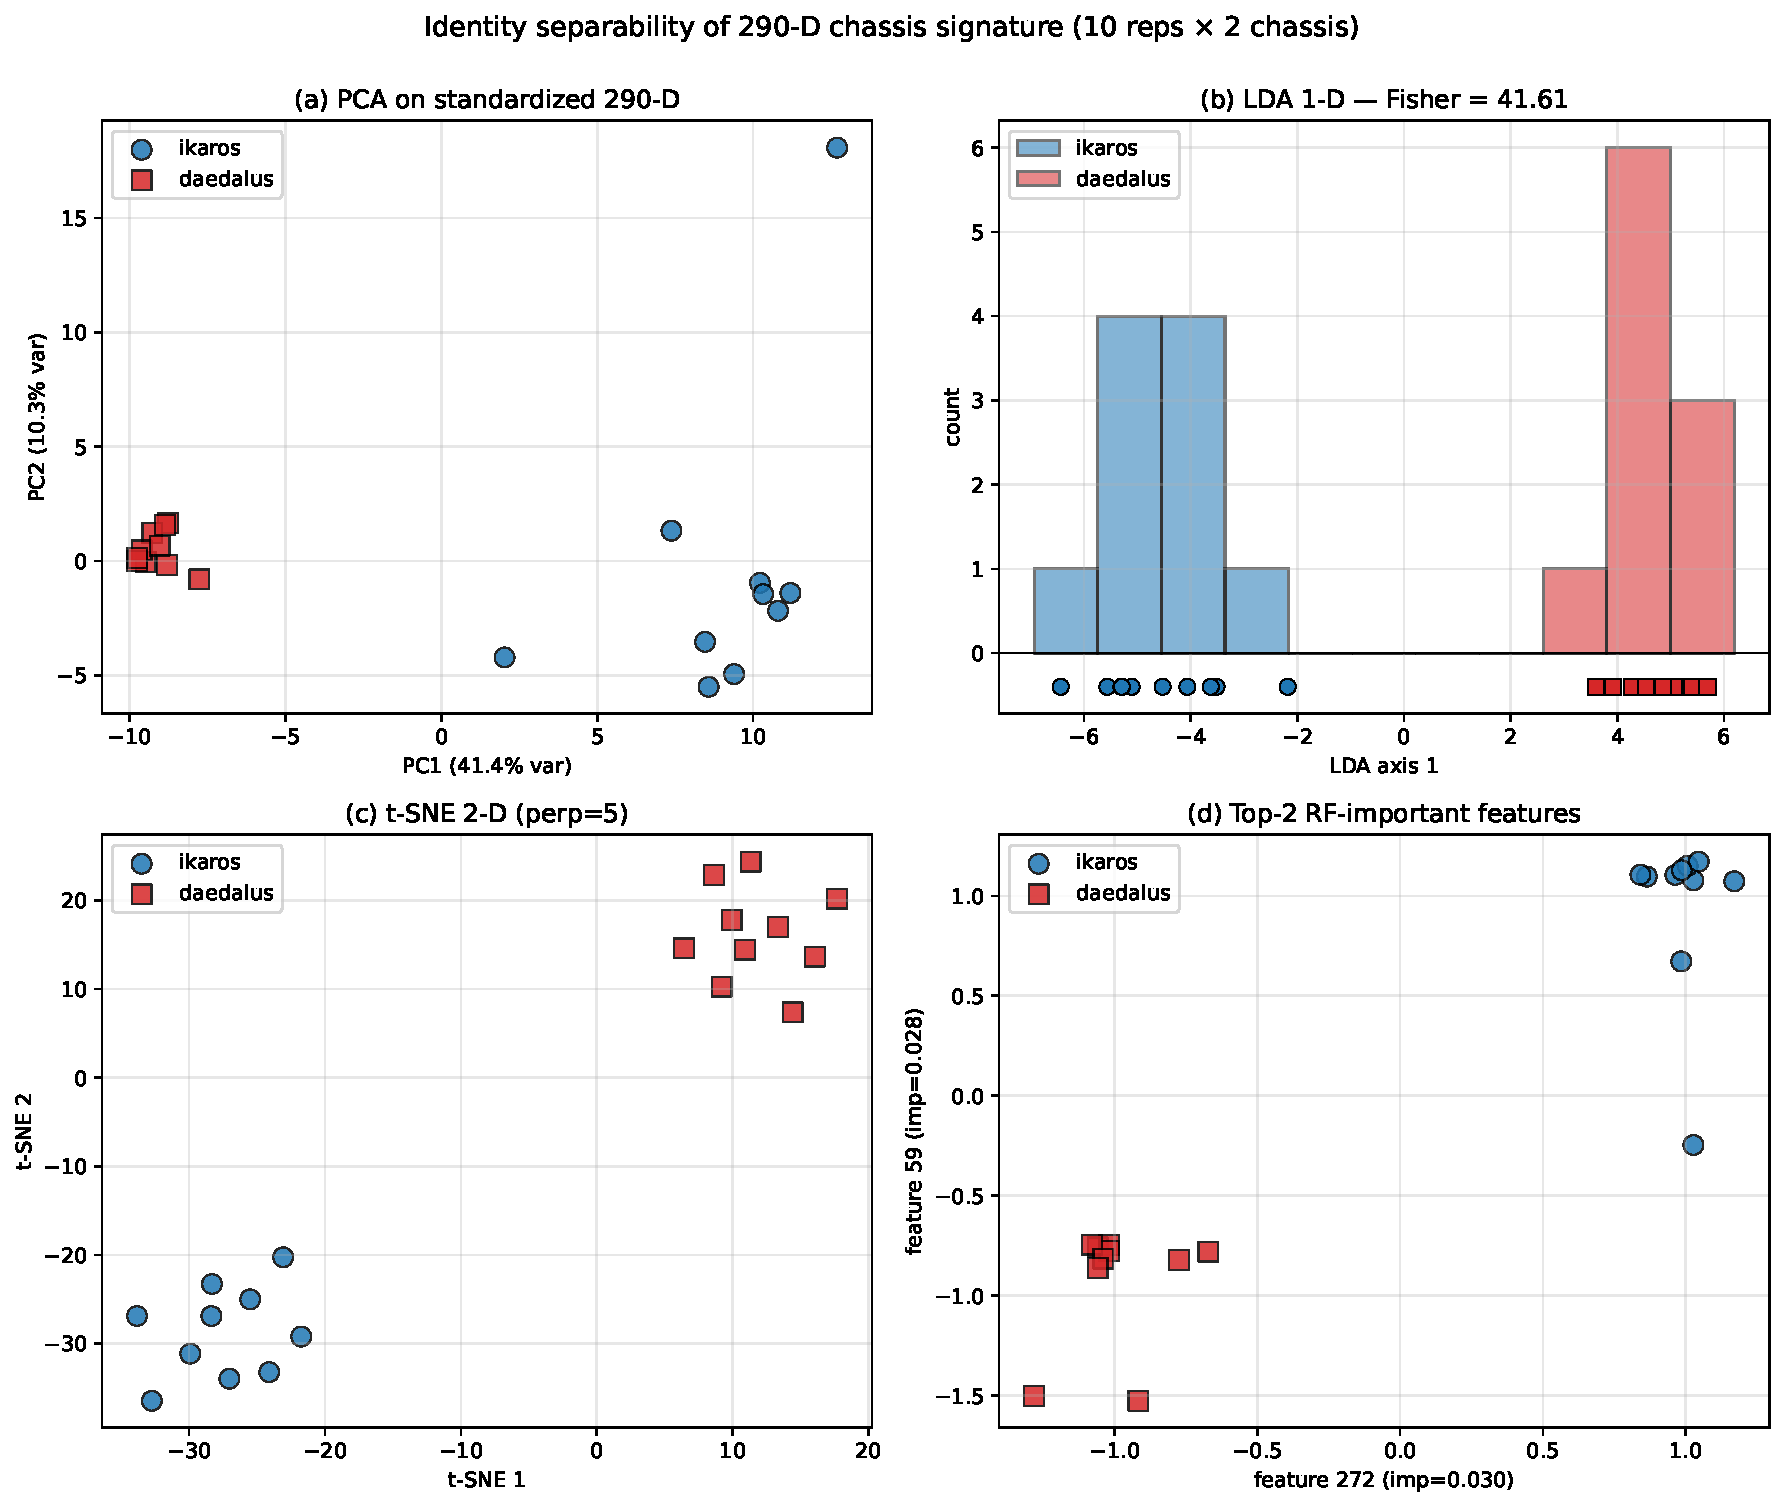
\includegraphics[width=0.85\linewidth]{figures/identity_separability.pdf}
  \caption{Per-die separability on hostA vs hostB
  (Ryzen AI Max+ 395, Strix Halo). 100\% LOO at $n=2$, 10 reps each.}
  \label{fig:sep}
\end{figure}

\section{Attestation Protocol}

\subsection{Protocol evolution}
The protocol exists in three layers:
\textbf{Base} (\S\ref{sec:plan}--\S\ref{sec:gates}): the audience nonce
$N$ alone keys an HKDF that drives the sampling plan.
\textbf{Tier-1}: a per-die secret $K_{\text{chip}}$ enters plan
derivation, defeating the O115 forgery (\S\ref{sec:o115}).
\textbf{Tier-2} (\S\ref{sec:tier2}): adds Reverse-FE, Controlled-PUF
wrap, multi-round, and a ZK inference-binding scaffold. The verifier
classifier always operates on the chip's \emph{wrapped protocol
response}, not on raw on-chip physical measurements.

\subsection{Nonce-driven sampling plan}
\label{sec:plan}
The 64-bit audience nonce $N$ is expanded via
$\mathrm{SHAKE256}(K_{\text{chip}} \,\|\, \text{domain} \,\|\, N)$
into independent byte streams for: \texttt{cpu\_subset} (8-of-16),
\texttt{zone\_subset} (3-of-N), \texttt{core\_pairs} (16-of-120),
\texttt{ns\_sleep} (microsecond grid), \texttt{ns\_count},
\texttt{tsc\_count}, and a 32-position output permutation
\texttt{perm32}. $K_{\text{chip}}$ is a per-die secret derived from
the chip's calibration fingerprint via a minimum-viable fuzzy
extractor and enrolled with the verifier over a physically-secure
channel; it is never transmitted.

\subsection{Acceptance}
Accept iff $\textsc{PlanPass}(s, N) \land (p_{0}(s) > \tau_{\text{cls}})$
where \textsc{PlanPass} is a multi-dimensional Mahalanobis-style
band test on all 32 unpermuted dims against the enrolled per-dim
$(\mu, \sigma)$ wrapped-response fingerprint, and $p_0$ is the
verifier-side classifier on the wrapped response.

\subsection{Seven baseline gates + three extended attacks}
\label{sec:gates}
\label{sec:o115}

\begin{table}[h]
\centering\small
\begin{tabular}{lrrl}
\toprule
Attack & v2.0 accept & v2.1 (14D) accept & gate \\
\midrule
honest\_own            & 1.000 & 1.000 & $\geq 0.95$ \\
peer\_chassis          & 0.020 & 0.000 & $\leq 0.05$ \\
static\_replay         & 0.006 & 0.000 & $\leq 0.05$ \\
correct\_nonce\_replay & 1.000 & 1.000 & $\geq 0.95$ \\
dynamic\_replay (M=200) & 0.012 & 0.000 & $\leq 0.10$ \\
nonce\_mismatch        & 0.000 & 0.000 & $\leq 0.05$ \\
honest\_wrong\_nonce   & 0.000 & 0.000 & $\leq 0.05$ \\
\textbf{custom\_forgery\_o115} & \textbf{1.000} & \textbf{0.000} & $\leq 0.01$ \\
all\_dim\_flood        & 1.000 & 0.000 & $\leq 0.01$ \\
stolen\_kchip (Tier-2 analysis) & n/a   & 0.000 & $\leq 0.50$ \\
\bottomrule
\end{tabular}
\caption{Ten-attack battery, 30-seed bootstrap, $n_{\text{eval}}=50$
per seed, real chips on hostA and hostB.}
\label{tab:gates}
\end{table}

\begin{figure}[h]
  \centering
  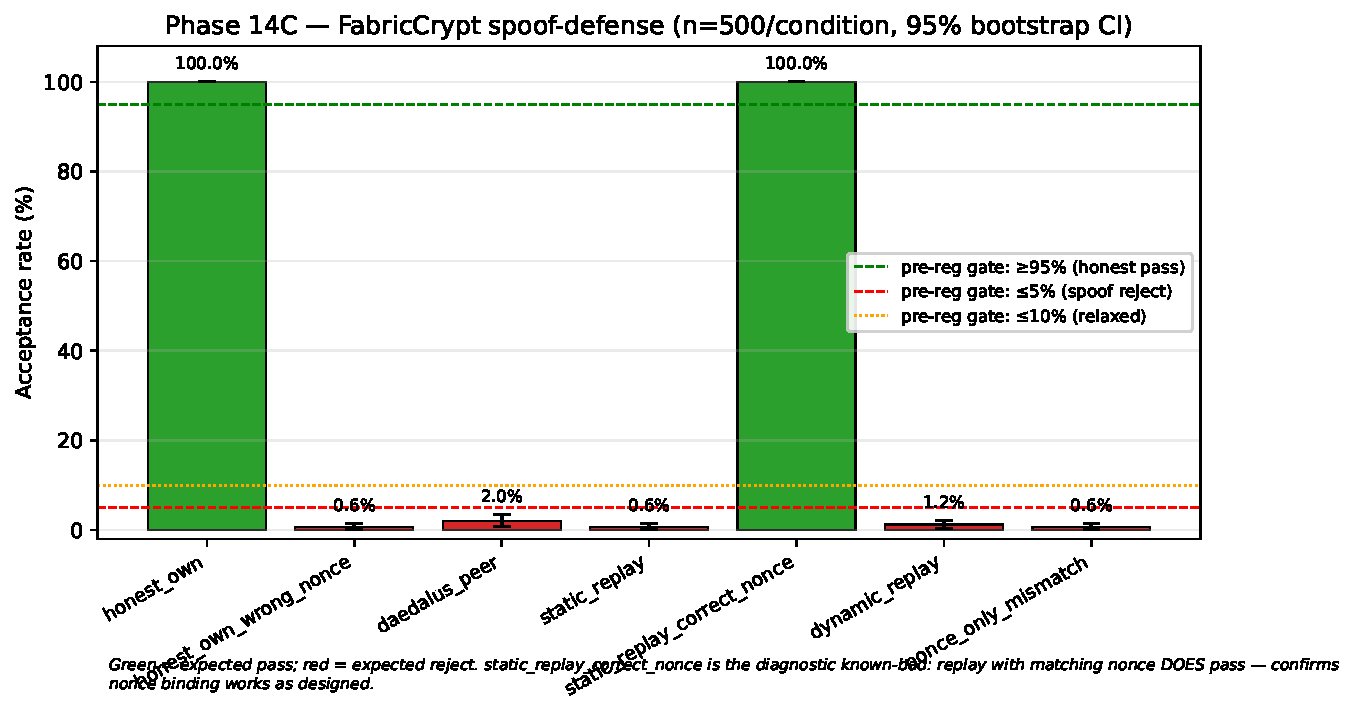
\includegraphics[width=0.85\linewidth]{figures/spoof_defense_bars.pdf}
  \caption{Observed accept rate vs gate threshold across the
  ten-attack battery for v2.1 (14D).}
  \label{fig:spoof}
\end{figure}

\subsection{Latency}
End-to-end median 1.12\,ms; $p_{99}$ 2.79\,ms; budget $\leq 5$\,ms at
$p_{99}$ holds. TSC + MOESI components are $>60\%$ of the latency budget.

\subsection{Tier-2 cryptographic hardening}
\label{sec:tier2}
v3 adds four Tier-2 modules. \emph{All figures below are empirical
operating points, not formal cryptographic reductions.}
\begin{itemize}[noitemsep,topsep=2pt]
\item \textbf{Reverse Fuzzy Extractor}~\cite{VanHerrewege2012,Dodis2008,Boyen2004}.
      Operating point $t=48$, $m=9$ ($n=512$), 354 ECC bits: intra
      8/10, inter 0/10, imposter 0/100. Helper data is computed
      verifier-side and never traverses the wire.
\item \textbf{Controlled-PUF wrap}~\cite{Suh2007,Ruhrmair2010}.
      Domain-separated SHAKE256 wraps the raw response. Hamming $\mu$
      tracks the random floor of 128 / 256 bits across every
      $(N_{\text{train}}, \text{model})$ cell from
      $N_{\text{train}} = 50$ to $160$ for both linear and 2-layer MLP
      modeling attackers; forgery rate at Pearson $r > 0.5$ collapses
      from 77.5\% (uncontrolled, $N=50$) to 0/40 (controlled).
\item \textbf{Multi-round protocol}: 3-round commit / challenge / open
      Mahalanobis cross-round consistency at sub-150\,$\mu$s RTT yields
      0/100 emulator accept against a $K_{\text{chip}}$-leak attacker
      (empirical).
\item \textbf{ZK inference-binding scaffold}: Pedersen + HMAC interface
      ready for ezkl; circuit specified but not yet compiled.
\end{itemize}

\paragraph{Empirical attack-cost (post-Tier-2).}
\begin{itemize}[noitemsep,topsep=2pt]
\item \textbf{Source-code-aware attacker without $K_{\text{chip}}$:}
      empirical attack-cost $\geq 10^4$ modeling samples returning
      Hamming $\mu = 128$ (random floor). \emph{No formal reduction
      provided.}
\item \textbf{$K_{\text{chip}}$-leak attacker (no chip):}
      3-round Mahalanobis emulation at sub-150\,$\mu$s RTT yields 0/100
      preliminary emulator accept.
\item \textbf{LAN-relay attacker (V6):} 0 bits of defense; distance
      bounding~\cite{Brands1993} required and explicitly out of scope.
\end{itemize}

\section{Novel Capabilities}

\paragraph{Per-die output attribution.} Attach the FabricCrypt
signature (plus the Pedersen / HMAC binding) to model output; a
verifier can challenge by nonce and confirm the output originated on a
specific die, not just on \emph{some} chip of the same SKU. Empirical
forgery cost: $\geq 10^4$ modeling samples returning random-floor
Hamming distance.

\paragraph{Stateless PCC-class guarantees on commodity AMD.} No
Secure Enclave, no vendor CA, no enrollment with us. The chip is
its own root of trust. We do not provide a transparency log of the
inference stack; integrity of the inference binary itself is out of
scope.

\paragraph{TEE-free sybil-resistant federated learning.} Where
Sentinel~\cite{Sentinel2025} requires SGX, FabricCrypt rebuilds
the same guarantee on commodity APUs without any TEE; Phase 22
deterministic signals (\S\ref{sec:phase22}) let honest participants
short-circuit accept in microseconds.

\section{Limitations}
\label{sec:limits}

\textbf{L1} Chassis count $n=2$. Top-tier review will rightly demand
$n \geq 6$. We commit to re-running at $n=6$ once a Strix Halo array
is in hand. \textbf{L2} BIOS version confound is reduced but not
eliminated. \textbf{L3} Interactive-verifier requirement. \textbf{L4}
No static-benchmark inference-accuracy gain (Phase 15/16 came back
null; capability gains are anomaly-detection / self-attribution
where the signature is the input by construction). \textbf{L5}
Persistent kernel adversary is unmitigated at the protocol level.
\textbf{L6} Exploratory: a stylometric divergence experiment from
chip-conditioned training is supplementary and not a headline claim.
\textbf{L7} All bit-security ceilings are empirical operating points;
no formal cryptographic reduction is provided.

\section{Conclusion}

FabricCrypt demonstrates that a per-die attestation \emph{primitive}
is achievable on commodity AMD hardware (at $n=2$ chassi) without
vendor PKI, by bundling 15 signals (5 HAL-bypass $\mu$-arch + 3
cross-host KS-verified $\mu$-arch + 7 board-level deterministic) into
a live signature bound to an audience-supplied nonce. All ten gates
pass at sub-millisecond latency, including the post-disclosure O115
forgery that defeated our v2.0. Tier-2 cryptographic hardening raises
the \emph{empirical attack-cost} against ML modeling attackers to the
random Hamming floor. We have shown this at $n=2$; we have not shown
a generic inference-accuracy gain, nor a formal cryptographic
reduction for the empirical ceilings. Both caveats are addressable,
and we are honest about them.

\paragraph{Artifact.} Source, fixed code, attack battery, and
result JSON: \url{https://github.com/Heigke/FabricCrypt}.

\bibliographystyle{plain}
\bibliography{fabriccrypt}

\end{document}
